\chapter{Evaluation of the ICE--Model}\label{modelanalysis}
We now have a complete geomtrical representation of the ICE model as well as
 the analytical expressions $u_0$ and $u_L$ that describe the membrane displacements
in spatial detail as a function of direction and frequency. In this chapter we will use these variables
to further study the features and predictions of our model and compare them with experimental results. In
order to completely explain the obeservations, we will also need to estimate certain physical parameters
like membrane eigenfrequency and quality factor that are important to our analysis but haven't been
experimentally measured.

The main body of this chapter proceeds in Sec. \ref{localizationsection} directly from the definitions given in \eqref{ipsimembranefull}
and \eqref{contramembranefull}. We will begin by assigning numerical values to the model parameters that have been defined
in the previous chapter. This will be done in Sec. \ref{parameterestimation}.
In Sec. \ref{hearingcuessection} we will define and study the two main quantities that serve as important localization
cues - the Internal Time Differences (iTDs) and the Internal Level Differences (iLDs). These values model the
neural subtraction taking place in the animal's brain which is the final step in localization.
In Sec. \ref{pressuredistchapter} we will
briefly discuss the pressure distribution profile and eigenfrequencies of the mouth cavity.
Finally, in Sec \ref{vibrationpatternchapter} we will compare the experimentally determined vibration pattern
of the Tokay gecko's eardrum with that of our model's eardrum - the aim being to justify our choice for the
geometry of the membrane.

In order to underline the fact that our model is universal model for internally coupled ears and not
specialized to single species, we will compare our results for two gecko species - \textit{Hemidactylus frenatus}
or the common house gecko and the Tokay gecko. At the end of the chapter we will have an understanding of the advantages of a coupled system of ears as opposed
to a pair of independent ears. We will also have an idea about the frequency regimes that correspond to the use
of iTDs and iLDs in localization.


\section{Sound Localization Using the ICE Model}\label{localizationsection}
In order to understand the estimation of 
these quantities we should first acquaint ourselves with some experimental details. As already mentioned in Sec. \ref{soundinput}, the geckos were placed in
an anechoic room. They were subject to $175$ms frequency sweeps (200-7500 Hz) at levels of 80-90 dB with the speakers placed at
a $1$m distance. The eardrum vibrations were then measured using laser-Doppler vibrometry with the point
of measurement at the tip of the extracolumella. The measured values correspond to the displacement velocity of the membrane at this point.  
In our analysis, the point corresponding to the tip of the extracolumella is stationary and cannot be used to compare the vibrations of the membranes. 
Instead, we use the total membrane vibrations defined in the previous chapter which are given by,
\begin{equation}
 S^0=G^s_{ipsi}p_0+G^s_{contra}p_L,\qquad S^L=G^s_{ipsi}p_L+G^s_{contra}p_0
\end{equation}
where we've used the ipsi- and contralateral filters defined in \eqref{ipsimembranetotal} and \eqref{contramembranetotal} and the
inputs have the form
\begin{equation}\label{newsoundinput}
 p_0=pe^{j\omega t} e^{-\Delta/2},\qquad p_L=pe^{j\omega t} e^{\Delta/2},\qquad \Delta=1.5kL\sin\theta.
\end{equation}
These quantities accurately
represent the response of the membrane to external stimuli and only depend on direction and frequency. We now define the displacement ratio of
the membranes,
\begin{align}
 \frac{S_L}{S_0}&=\frac{1+\eta e^{1.5jkL\sin\theta}}{\eta+e^{1.5jkL\sin\theta}}\\
 \mbox{where, }\eta&=\frac{G^s_{ipsi}}{G^s_{contra}}=\frac{1}{\frac{\pi a^2_{cyl}\Lambda}{\rho c\omega}\sin kL-\cos kL}
\end{align}
after using the appropriate formulas and simplifying the expressions.
\section{Parameter Estimation}\label{parameterestimation}
In our study we are primarily concerned with hearing in geckos. We will be using
parameters (interaural separation, tympanum area etc.) from \textit{Hemidactylus frenatus}, the common house gecko
\cite{dalsgaardmanley2} and the Tokay gecko \cite{dalsgaardmanley1}, \cite{dalsgaardtangcarr}. In order to proceed
with our evaluation of our model, we will need to assign appropriate numerical values to the parameters we have
defined in \ref{parametertable}. Some of the parameters can be directly taken from their measured values whereas
the rest will need to be estimated indirectly. 

For the head width/interaural distance ($L$), cavity volume ($V_0$), the density of the membrane ($\rho_m$) and its thickness ($d$)
we can use the directly measured values. The radius of the cylinder ($a_{cyl}$) can be calculated from the first two quantities
using \eqref{cylinderradiusformula}. 
As we've already seen in Fig. \ref{tympanummodel}, the realistic tympanic membrane is an ellipsoid rather than a perfect circle therefore the radius of our tympanum will
instead be estimated from the area of the membrane as $a_{tymp}=\sqrt{A/\pi}$. The extracolumella angle ($\beta$) is also estimated similarly.

The parameters that require an indirect estimation are the first membrane eigenfrequency ($\omega_{01}$) and
its quality factor $Q$ which effectively gives us the membrane damping. These quantities are difficult to directly measure and instead
have to be estimated from experimental results and the frequency response of the system.
The calculated and estimated parameters are listed for both the species in Table \ref{geckogeometricparams}.

\vspace{\baselineskip}
\noindent
\begin{minipage}{\linewidth}
\renewcommand{\arraystretch}{1.3}
%\caption{Parameters and Functions used in the ICE Model} \label{parametertable} 
\centering
\captionof{table}{ICE Model geometry Parameters for the common house gecko (Hemidactylus frenatus) and the Tokay gecko.}\label{geckogeometricparams}
\begin{tabular}{|p{8.5 cm} | c | c|}
\hline
Parameter name & Hemidactylus & Tokay gecko\\
\hline
Length of the cylinder or interaural distance, L & $10$mm & $25.6$mm\\
Radius of the tympanic membrane, $a_{tymp}$& $1.5$mm & $3.0$mm\\
Fundamental frequency (first eigenfrequency) of the tympanic membrane, $\omega_{01}$ & $3200$Hz & $1700$Hz\\
Quality factor of the tympanum, $Q$ & $1.3$ &  $1.7$\\
Density of the membrane material, $\rho_m$ & $1$mg/mm$^3$ & $1$mg/mm$^3$\\
Thickness of the membrane, $d$& $8\mu$m & $10\mu$m\\
Volume of the cavity, $V_0$ & $.32$ml & $3.5$ml\\ 
Extracolumella angle, $\beta$ & $\pi/25$ & $\pi/25$\\
Cylinder radius calculated from $V_0$ and $L$ using the formula given in \eqref{cylinderradiusformula}, $a_{cyl}$ & $\sim 6.6$mm  &$\sim 3.2$mm \\
\hline
\end {tabular}\par
\bigskip
\end{minipage}

As we can see, the house gecko, with an interaural separation of $10$mm and mouth cavity volume of $.32$ml is a rather
small lizard. The Tokay gecko is the second largest gecko species (interaural separation of $25.6$mm and mouth cavity volume $3.5$ml, \cite{dalsgaardtangcarr}).
Thus we will demonstrate the scalability of our model with regards to hearing in animals with widely varying head widths and mouth cavities. The geometric parameters, especially
the head width and the membrane eigenfrequencies put important limits on the ``hearing range'' of our model as we will see in the upcoming section.

\subsection{Directional Hearing Cues}\label{hearingcuessection}
The iTD and iLD can be seen as the output of the ICE system with $p_0$ and $p_L$ as inputs.
In contrast to the Interaural Time and Level Differences (ITD and ILD) are entirely determined 
by the inputs to the two ears. The ITD is defined as the time sound takes to travel across
the head width and is given by $ITD=L/c$. It therefore corresponds to the phase difference
between the vibrations of the eardrums without coupling and diffraction effects. 

The level difference corresponds to the 

\subsubsection{Transmission Gain}

\subsubsection{Internal Time Difference}

\subsubsection{Internal Level Difference}

\section{Cavity Pressure Distribution}\label{pressuredistchapter}

\section{Spatial Vibration Pattern of the Membrane}\label{vibrationpatternchapter}
We begin our analysis by evaluating the variation of the spatial vibration pattern of the tympanic membrane
with frequency. The tympanic vibration pattern was first measured experimentally by Manley \cite{manleygecko1}
for a \textit{Tokay gecko} and was found to have the strongest response at around 1kHz. The measured vibration patterns
are shown on the left in Fig. \ref{manleygeckotympanum}. Manley measured the vibration amplitude for eight locations on the membrane and measured the pattern
seen on the left of Fig. \ref{manleygeckotympanum}. As we can see, at around $4$kHz, the vibration pattern
distinctly develops two maxima - something that would not happen to a centrally loaded tympanum except
at frequencies well beyond the hearing range of geckos.

\begin{figure}[ht!]
 \centering
 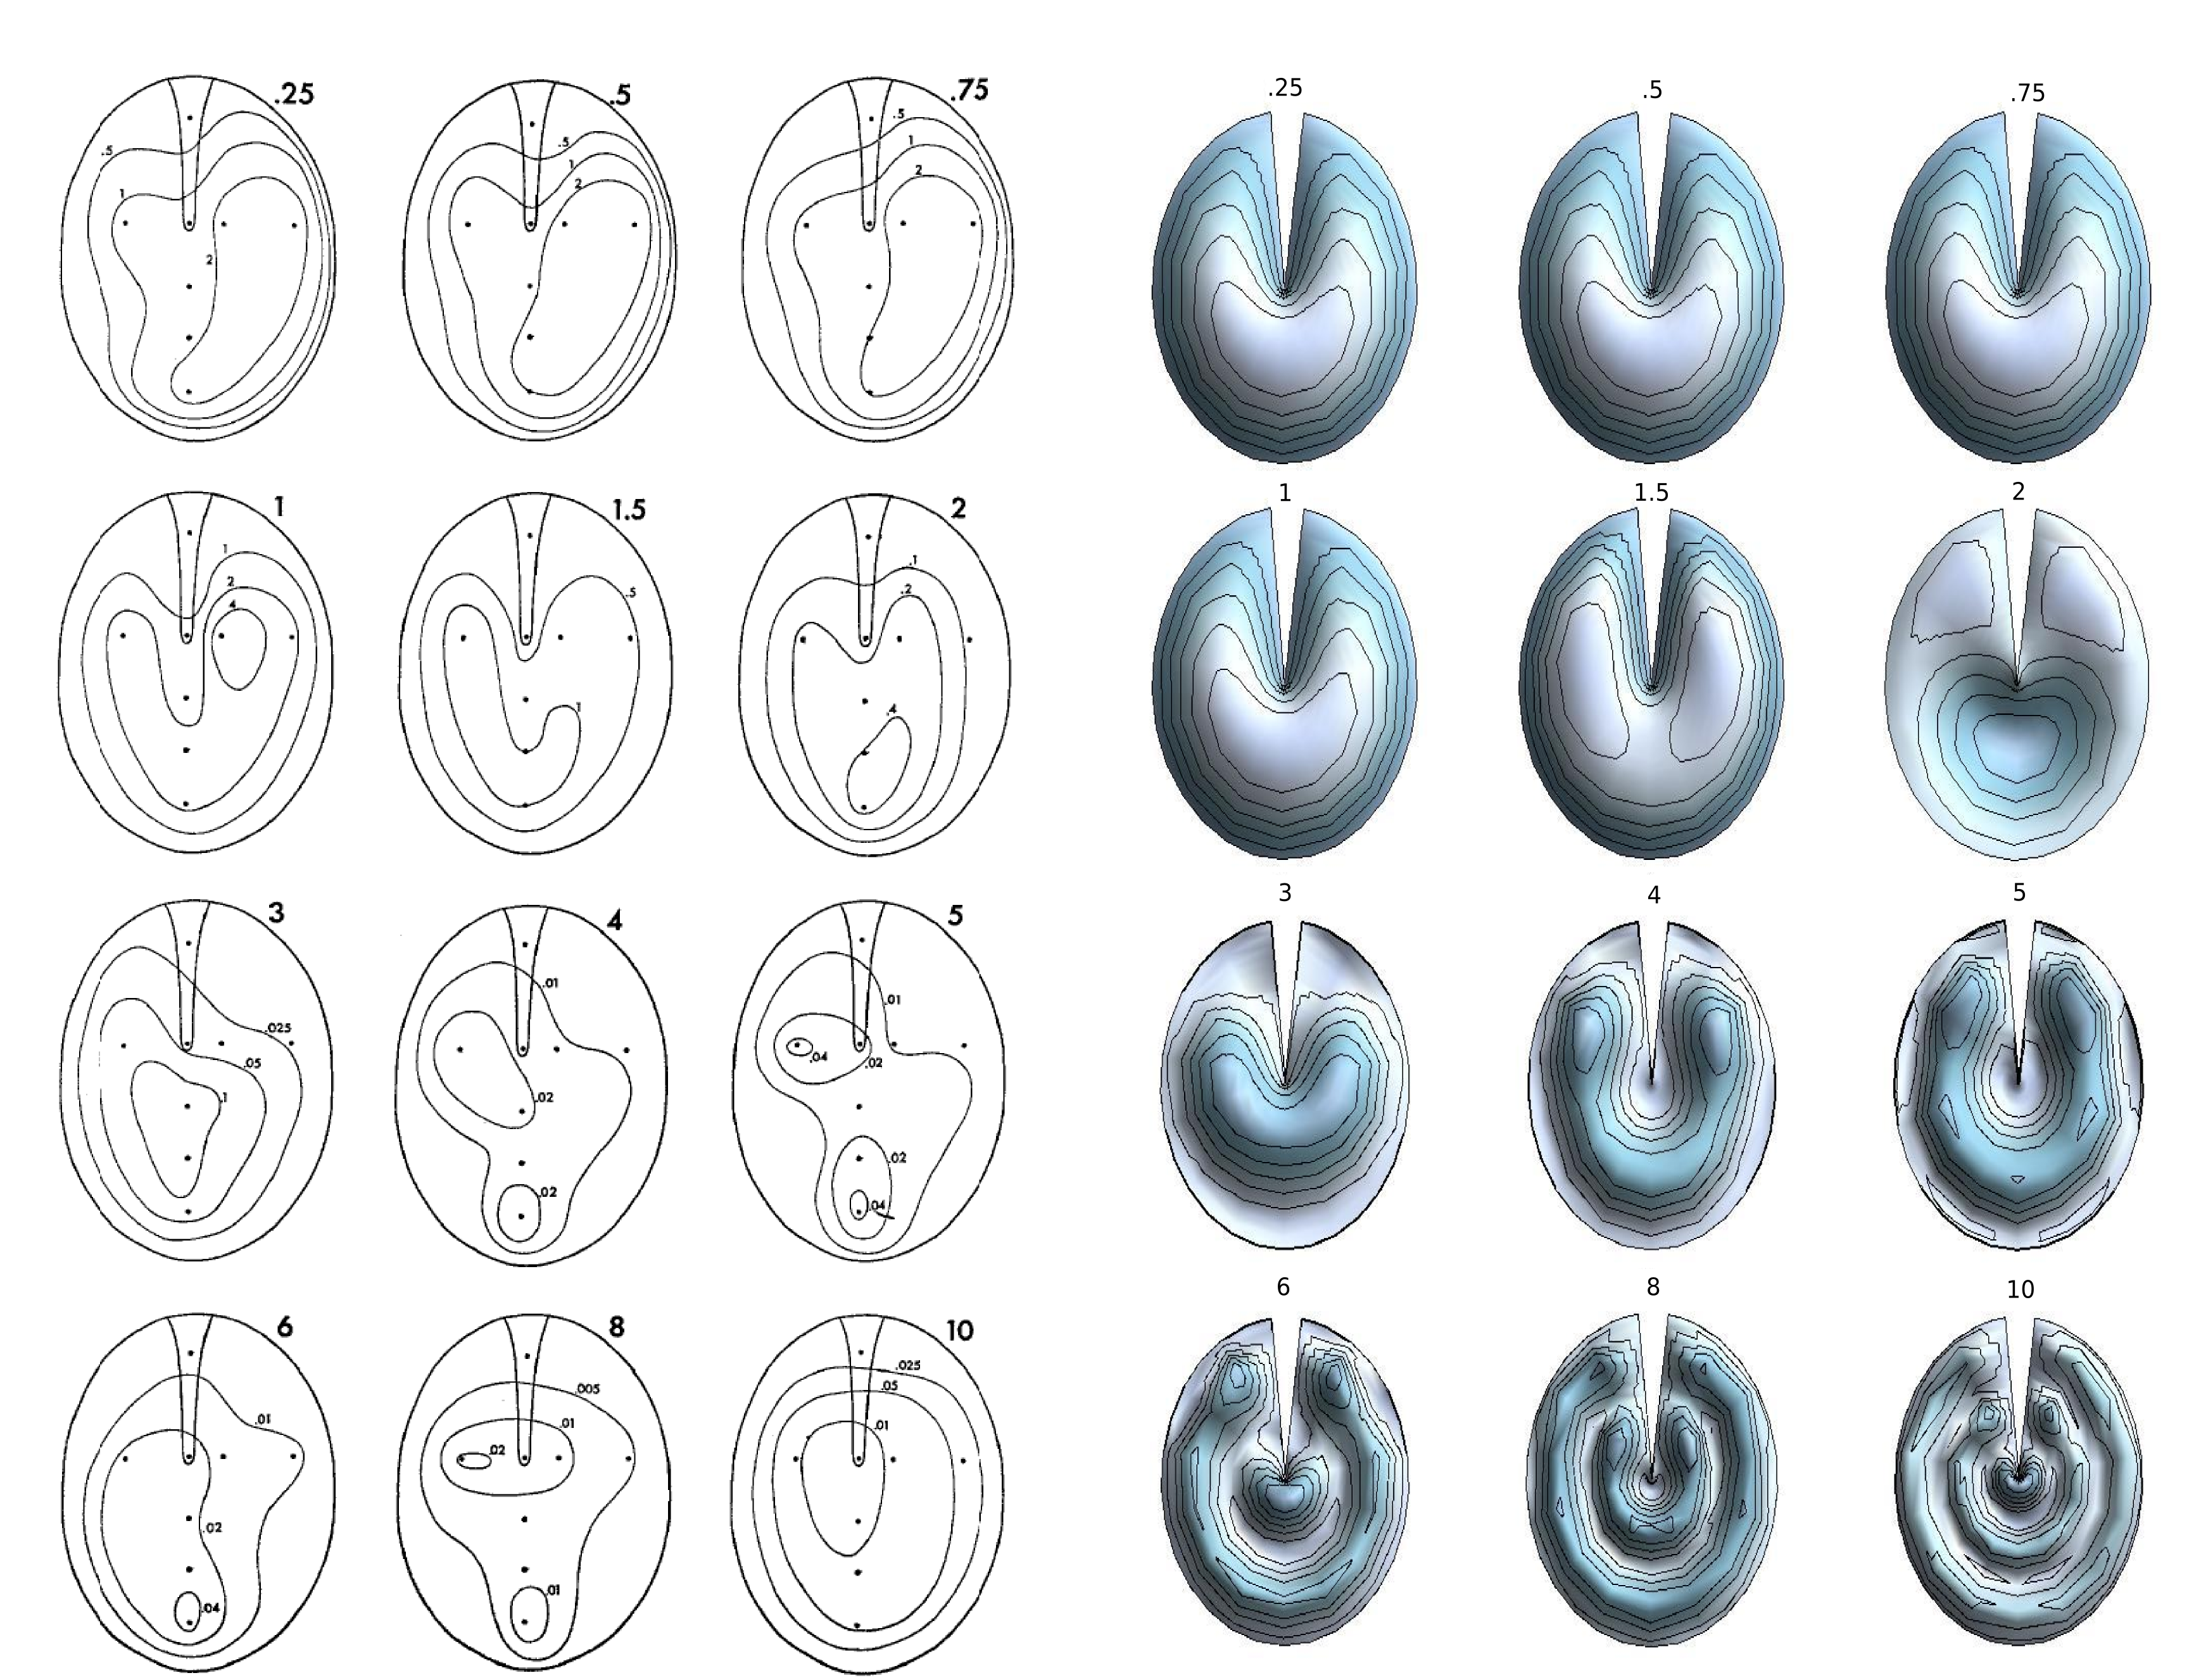
\includegraphics[width=1.0\linewidth]{Diagrams/manleymodelcomparison.png}
 \caption[Tokay gecko tympanum vibration profiles.]{Experimental membrane vibration patterns of the Tokay gecko dependent
 on sound frequency varying from $.5$kHz to $10$kHz. Data taken from \cite{manleygecko1}.}
  \label{manleygeckotympanum}
\end{figure}

In order to compare our model with the experimental results, we plot the response of the ipsilateral membrane in our cylindrical ICE model 
calculated using \eqref{ipsimembranefull}. The input was chosen to be purely ipsilateral, meaning $p_L=0$. 
This is illustrated in Fig. \ref{manleygeckotympanum} (right) for the same frequency range as in the experimental data. The ipsilateral input was chosen to have unit amplitude and the model parameters used are given
on the right most column of Table \ref{geckogeometricparams}. The omitted region corresponds to the extracolumella. 

The asymmetric nature of our membrane vibration pattern is a result of our chosen geometry.
Mathematically this is a result of the fact that a uniform pressure (on the membrane surface) on a full circular membrane only couples to the circularly symmetric $J_0$ modes.
In the case of the sectoral membrane however, the uniform pressure couples to all the eigenmodes resulting in a more complex pattern.
As a qualitative reproduction our model is very accurate but for a full quantitative analysis, we would 
need to account for the motion of the extracolumella. Moreover, the full mechanics of the extracolumella would 
also include its flection at higher frequencies.
% \begin{figure}[ht!]
%  \centering
%  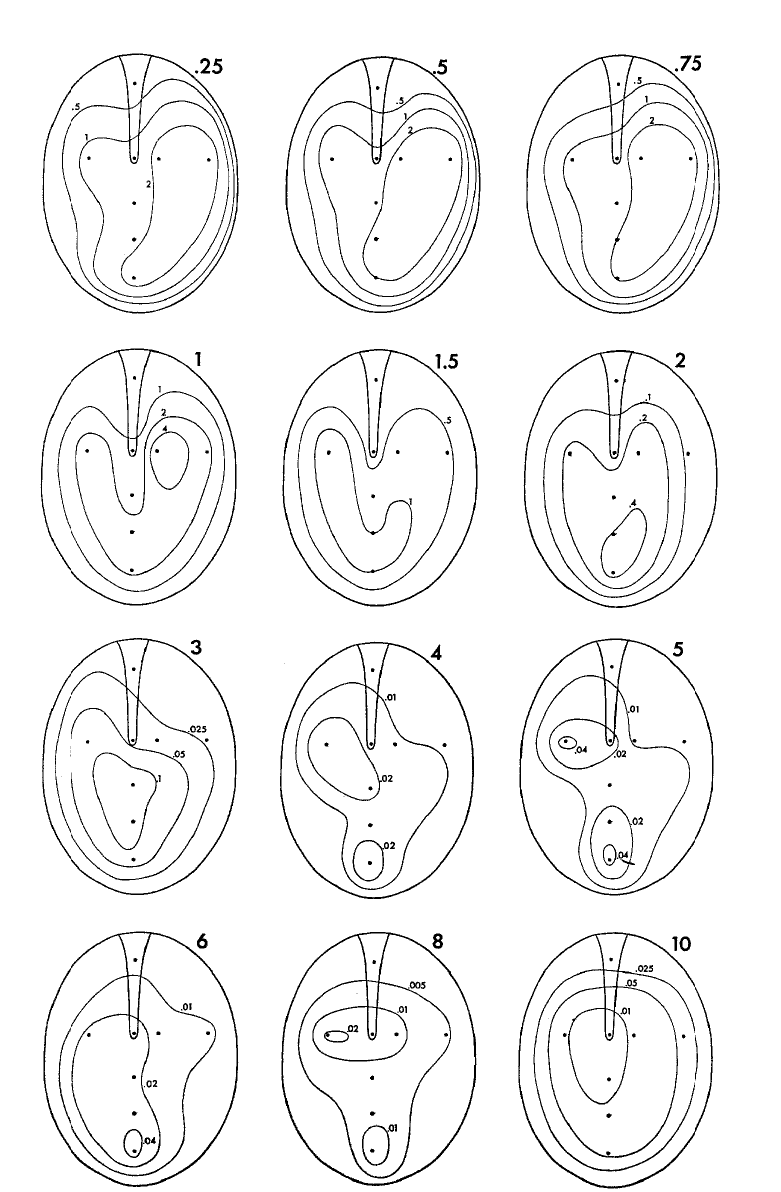
\includegraphics[width=.5\linewidth]{Diagrams/manleygeckoear2.png}
%  \caption[Tokay gecko tympanum vibration profiles.]{Experimental membrane vibration patterns of the Tokay gecko dependent
%  on sound frequency varying from $.5$kHz to $10$kHz. Data taken from \cite{manleygecko1}.}
%   \label{manleygeckotympanum}
% \end{figure}

% \begin{figure}[ht!]
%  \centering
%  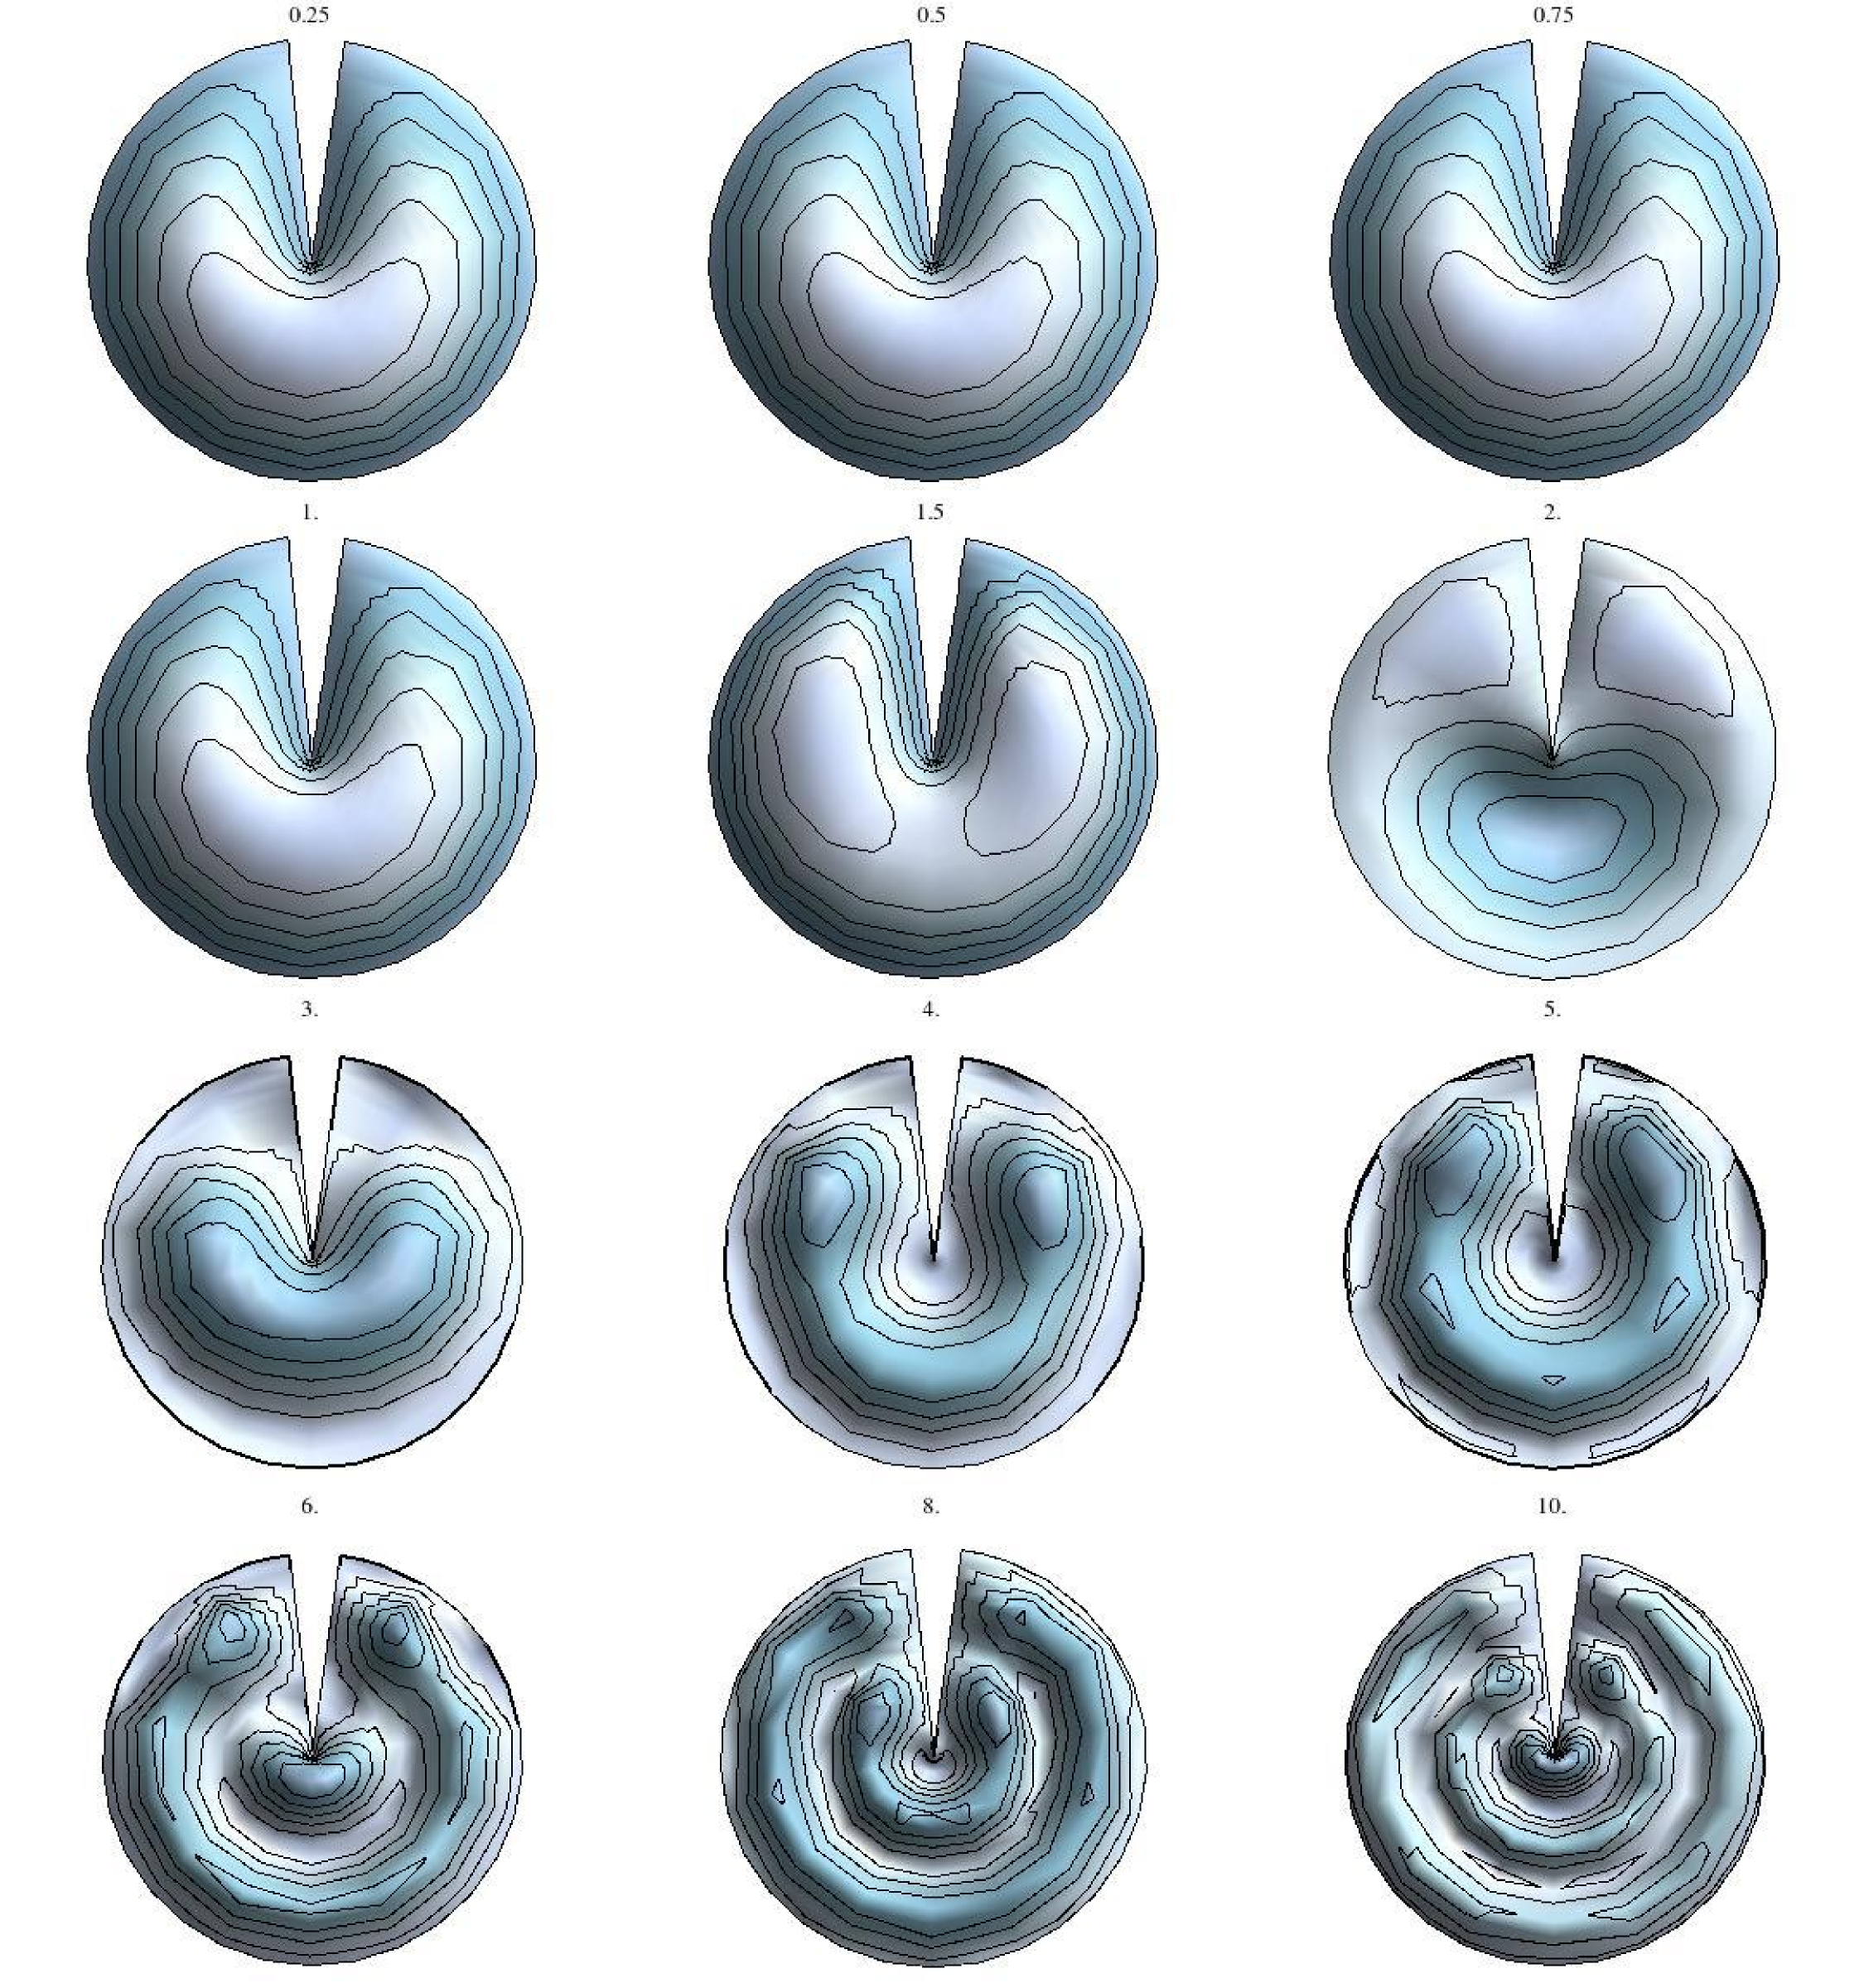
\includegraphics[width=.75\linewidth]{Diagrams/SectorMembraneModes/sector_membrane_all.png}
%  \caption[Sectoral membrane vibration profiles.]{Vibration patterns of a sectoral membrane
%  of radius $2.2$mm on sound frequency varying from $.5$kHz to $10$kHz. Compare with fig. \ref{manleygeckotympanum}}
%   \label{sectormembraneprofile}
% \end{figure}